\section{Nuclear Reaction Differential Cross Sections}
Figures \ref{fig:sig_rt} and \ref{fig:sig_r} show plots of the total and differential nuclear-reaction cross sections for energetic deuterons colliding with tritons and producing energetic neutrons, that is, 
\begin{equation}
    \sigma_{D,T \rightarrow n}(E^{\prime} \rightarrow E; \mucm).
\end{equation}
This DT nuclear-reaction collision also results in the production of an energetic $\alpha$-particle, but this cross section is not directly tabulated in the ENDF files and two-body kinematics are needed to calculate the corresponding differential cross section. From Figure \ref{fig:sig_rt}, the DT fusion reaction clearly has a threshold for reaction of about 0.02 MeV and a peak for incident deuterons of 0.1 MeV. Furthermore, looking at Figure \ref{fig:sig_r}, the neutrons that are produced are almost nearly isotropic in angle. While this DT nuclear-reaction cross section only represents one possible type of charged particle collision, the general comment that can be made is that charged-particle nuclear-reaction differential cross sections are not highly peaked and that these types of collisions have large MFPs when compared to the Coulomb differential cross sections.

\begin{figure}[!htb]
    \centering
    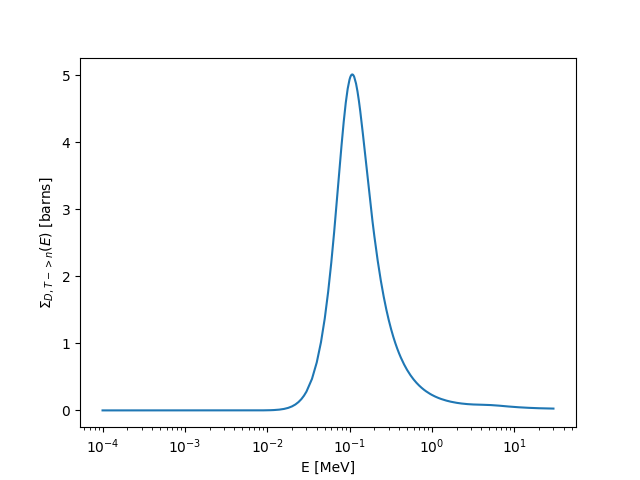
\includegraphics[scale=0.75]{../figures/boltzmann_model/DT_TotalReactionXS.png}
    \caption{Total nuclear-reaction cross section for $D+T \rightarrow n$}
    \label{fig:sig_rt}
\end{figure}

\begin{figure}[!htb]
    \centering
    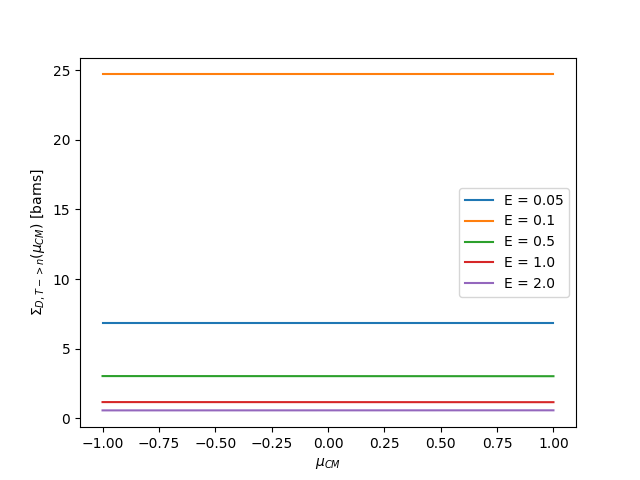
\includegraphics[scale=0.75]{../figures/boltzmann_model/DT_ReactionXS.png}
    \caption{Nuclear-reaction differential cross section for $D+T \rightarrow n$}
    \label{fig:sig_r}
\end{figure}